\section{MBRM: A MicroBlog Retrieval Model}
\label{MBRM-section}
In the previous section, we discussed a number of problems faced by state of the art retrieval models when dealing with microblogs. We presented scarcity of TF and DL as a source of high scoring differences amongst the spectrum of possible scores for a retrieval model. Additionally we started defining the requirements for a retrieval model to effectively handle microblog documents by better capturing their informativeness. These requirements can be summarised as: 

\begin{enumerate}
\item Higher DL should be regarded positively as authors of microblogs strive to fit as much content as possible within the character limits
\item Higher TF should be regarded negatively as high TF could be a result of spam messages, and normally TF revolves around 1-2
\item Score differences with respect to DL and TF should produce gentle slopes, to not penalise/promote unfairly documents with very little differences.
\end{enumerate}

Following these premises, we have designed a ``MicroBlogs Retrieval Model'', namely MBRM. MBRM is composed of two parts to deal with document based evidence. Then we attach the aforementioned part to an IDF component which represents the collection's information. Similarly to the formulation of BM25, the two main components of MBRM deal with document length and query term frequency. The first component deals with the document length and is given by the following logistic distribution:

\begin{equation}
DLComp(DL)={\frac  {c_1}{1+{a_1\mathrm  e}^{{-b_1DL}}}}
\end{equation}

where \(a_1, b_1\) and \(c_1\) are parameters to control the growth, maximum and starting point of the distribution. Secondly, the following component given by a gaussian distribution deals with the effect of TF over the final score produced by MBRM:

\begin{equation}
TFComp\left(TF\right)=a_2e^{-{\frac {(TF-b_2)^{2}}{2c_2^{2}}}}
\end{equation}

where \(a_2, b_2\) and \(c_2\) are similar parameters to those found in the previous function. These functions were chosen as they offer good control over the curves, and their values can be bound between 0 and 1 thus we do not need to normalise them. The final formulation for MBRM is given by: 

\begin{equation}
MBRM(D,Q) = \sum_{i=1}^{|Q|} (1-\alpha)*\text{IDF}(q_i) + \alpha * DLComp(|D|) * TFComp(q_i)
\end{equation}

which can be also expressed as:

\begin{equation}
MBRM(D,Q) = \sum_{i=1}^{|Q|} (1-\alpha)*\text{IDF}(q_i) + \alpha * \left({\frac  {c_1}{1+{a_1\mathrm e}^{{-b_1DL(|D|)}}}} \right) * \left(a_2e^{-{\frac {(TF(q_i)-b_2)^{2}}{2c_2^{2}}}}\right) 
\end{equation}

\begin{table}[b]
	\caption{MBRM recommended parameter settings} 
	\centering
	\begin{tabular}{l|c} 	
		\hline
		\textbf{Parameter} & \textbf{Recommended values} \\
		\hline
		\centering					 
		$a_1$ & 1.5 \\
		$b_1$ & 0.3 \\
		$c_1$ & 1.0 \\
		\hline
		$a_2$ & 1.0 \\
		$b_2$ & 2.0 \\
		$c_2$ & 6.0 \\
		\hline
	\end{tabular}
	\label{recommended settings}
\end{table}

Figure \ref{microblogRM} shows a simulation of the behaviour of MBRM in terms of TF and DL. The parameters used to for both components (DLComp and TFComp) are shown in Table \ref{recommended settings}. In Figure \ref{microblogRM} we can observe how the values obtained on the TF axis decrease slowly for the initial values of TF, but rapidly accelerate in their descent to then settle near 0. This behaviour is similar to that of DFRee (Albeit smoother) in which the highest importance is given to low TF values $\sim2$ and then it is reduced. 
%High TF values are most likely than not associated with spam or unimportant documents, since actual users struggling to fit their content in the 140 characters limit are unlikely to repeat words. Although this is not always the case, thus the slow descent for low values of TF.

\begin{figure}
	\begin{subfigure}[]{0.5\textwidth}
		\caption{Doc. length (DL) and Term Frequency (TF)}
		\input{MBRM-GAUSS-TF}
		\label{microblogRM}
	\end{subfigure} 
	~
	\begin{subfigure}[]{0.5\textwidth}
		\vspace{-0.7cm}
		\caption{MBRM effects of $\alpha$ on each fold.}
		\hspace{0.5cm}
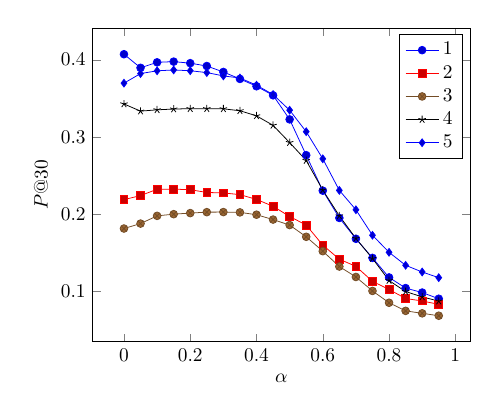
\begin{tikzpicture}[thick,scale=0.7, every node/.style={transform shape}]
\begin{axis}[
	xlabel={$\alpha$},
	ylabel={$P@30$}
]
\addplot coordinates {
	(0,0.4071)	(0.05,0.3895)	(0.1,0.3966)	(0.15,0.3975)	(0.2,0.3955)	(0.25,0.3918)	(0.3,0.3841)	(0.35,0.3751)	(0.4,0.3656)	(0.45,0.3539)	(0.5,0.3227)	(0.55,0.2764)	(0.6,0.2304)	(0.65,0.1951)	(0.7,0.1681)	(0.75,0.1434)	(0.8,0.1181)	(0.85,0.1043)	(0.9,0.0985)	(0.95,0.0905)
};

\addplot coordinates{	
	(0,0.2188)	(0.05,0.2241)	(0.1,0.2322)	(0.15,0.2324)	(0.2,0.2317)	(0.25,0.2281)	(0.3,0.2275)	(0.35,0.2253)	(0.4,0.2191)	(0.45,0.2102)	(0.5,0.197)	(0.55,0.1859)	(0.6,0.1599)	(0.65,0.1417)	(0.7,0.1324)	(0.75,0.113)	(0.8,0.1025)	(0.85,0.0908)	(0.9,0.0876)	(0.95,0.0832)
};

\addplot coordinates{
	(0,0.1814)	(0.05,0.1878)	(0.1,0.1978)	(0.15,0.2)	(0.2,0.2014)	(0.25,0.2026)	(0.3,0.2027)	(0.35,0.2023)	(0.4,0.1993)	(0.45,0.193)	(0.5,0.1859)	(0.55,0.1707)	(0.6,0.1521)	(0.65,0.1322)	(0.7,0.1187)	(0.75,0.1006)	(0.8,0.0853)	(0.85,0.0748)	(0.9,0.0716)	(0.95,0.0685)
};

\addplot coordinates{
	(0,0.3427)	(0.05,0.3334)	(0.1,0.3351)	(0.15,0.3361)	(0.2,0.3366)	(0.25,0.3366)	(0.3,0.3364)	(0.35,0.3339)	(0.4,0.3273)	(0.45,0.315)	(0.5,0.2927)	(0.55,0.2695)	(0.6,0.2312)	(0.65,0.1978)	(0.7,0.1686)	(0.75,0.1426)	(0.8,0.1141)	(0.85,0.0998)	(0.9,0.0929)	(0.95,0.0874)
};

\addplot coordinates{
		(0,0.3696)	(0.05,0.382)	(0.1,0.3856)	(0.15,0.3867)	(0.2,0.3857)	(0.25,0.3833)	(0.3,0.379)	(0.35,0.3763)	(0.4,0.367)	(0.45,0.3549)	(0.5,0.3346)	(0.55,0.3068)	(0.6,0.2717)	(0.65,0.2308)	(0.7,0.2057)	(0.75,0.1727)	(0.8,0.1506)	(0.85,0.1338)	(0.9,0.1251)	(0.95,0.1178)
};
\legend{$1$,$2$,$3$,$4$,$5$}
\end{axis}
\end{tikzpicture}
		\label{microblogRM-param}
	\end{subfigure} 
	\caption{MBRM: A Microblog Retrieval Model}
\end{figure} 

In terms of $DL$ we produce a soft increasing slope to account for increasing value assigned to more informative documents. Unlike $DFRee$, the slope is always incremental. The idea behind it being that the more terms in the microblog the more comprehensive it should be, as more information is encoded regardless of the character limitation.

In order to find the optimal value for the pondering value of $\alpha$ we divided the all the collections into 5 folds. For each of the folds we produced a P@30 result for a number of $\alpha$ values in the 0-1 range. These can be found in Figure \ref{microblogRM-param}. It can very easily be observed that the most optimal values for the mixing parameter $\alpha$ are near $0.20$.

Finally Table \ref{MBRMPerformance} shows the evaluation results obtained for MBRM in terms of Precision at different levels in comparison with IDF and DFRee. As it can be observed, the performance is always significantly superior than the baselines. The main difference with respect to IDF is obviously that it takes advantage of document statistics, where IDF does not. However the main difference with respect to DFRee is that documents longer than 15 terms are not penalised following the aforementioned rationale. 

These results not only demonstrate that we can make effective use of document statistics unlike previously thought by other authors \cite{naveed2011searching}, but also that the scope hypotheses still holds for small documents. In other words, the authors of the documents will attempt to encode as much information as possible even with the obvious document limitations. 

%This contradicts our findings in Subsection \ref{bm25case} however we believe that in the particular case of BM25, document length has a much more aggressive effect on the scores, thus resulting in a misleading behaviour.

\begin{table}[] 	
	  	  	\centering
	  	  	\caption{Performance of MBRM on all collections (Where * $p<0.05$ and ** $p<0.01$ respectively, with respect to IDF and DFRee)} 
	  	 	\begin{tabular}{l|c|c|c|c|c} 	  	 	
	  	 	\cline{2- 6}
	  	 	\multicolumn{1}{c}{}&\multicolumn{5}{c}{Precision} \\ 
	  	 	\cline{2- 6} &
	  	 	\textit{\textbf{@5}} & 
	  	 	\textit{\textbf{@10}} & 
	  	 	\textit{\textbf{@15}} & 
	  	 	\textit{\textbf{@20}} & 
	  	 	\textit{\textbf{@30}} 
	  	 	\tabularnewline
	  	 	\hline
	 	 	 DFRee  & 0.62 & 0.57 & 0.54 & 0.51 & 0.46 \\
	 	 	 IDF  & 0.62 & 0.57 & 0.53 & 0.51 & 0.46 \\
	 	 	 \hline
 	 	 	 \hline
  	  	 	 MBRM ($\alpha=0.20$)  & \textbf{0.64*} & \textbf{0.59*} & \textbf{0.56**} & \textbf{0.53**} & \textbf{0.48*} \\
	  	  	\hline
	  	  	\end{tabular}
	  	  	\label{MBRMPerformance}	
\end{table}


However, based on the statistically significantly better performance achieved by MBRM the verbose hypotheses seems not to hold, as authors capped by the character limitation. Thus documents are not generally longer due to style differences, or the verbosity of the author, but it is rather a reflection of the author's capacity to encode rich information in such limited constraints, which again aligns better with the scope hypotheses. And this is what we ultimately aimed to capture with our MBRM retrieval model.
